\chapter{Fundamental Blocks of the Research} \label{chapter_two}


\section{Image Stabilisation}
If the camera is not stationary during video capture the output video quality may degrade and it not look very good. Depending on the movements during capture, the may look very shaky or even the subjects of the video may not be properly visible. This is undesirable and can cause visual discomfort \citep{jia2012probabilistic}. The solution to this maybe to keep the camera steady by mounting it on stable tripod or a rigid object. But this is not practically possible all the time. There are various scenarios in which the camera may move around a lot and the movements may not be smooth at all e.g an action camera mounted on a helmet or a bicycle, a camera mounted on a car or a robot in wild or some move-able rig or robot arm. 

The motion of the camera can be high-frequency tremors due vibration of the mounting point or low frequency such as movement of handheld camera during walking \citep{dis_review}. Practically, in most of the video recording scenarios, the camera will have some movement. The goal of image stabilization is to create a output video with same visual content without the undesired movements. 

% Start: Image Stabilisation
\subsection{Types of Image Stabilisation}
To deal with such movements and to make the video stable various techniques exist. These techniques are grouped in two categories:

\begin{itemize}
\item Hardware Image Stabilization
\item Digital Image Stabilization  
\end{itemize}
There are techniques which combine both these methods and are called Hybrid Image Stabilization techniques.

The goal of each of these stabilization techniques is to estimate the motion and then do something to counteract that motion. Let' see how these movements are countered in each of these techniques.

\subsubsection{Hardware Image Stabilisation}
Hardware image stabilization (HIS) at its core means moving the lens or the image sensor or the camera setup itself to counteract these movements while recording the video in the first place. The movements of camera can be minimised by the use of mechanical stabilizers like tripods or dollies \citep{5995525}. The use of electronic gimbals for video recording has also increased recently for both professionals and hobbyists. Video can also be stabilised by varying the optical path between lens and the image sensor. This is generally achieved by using electronic motors and IMU sensors to move around the lens or the image sensor or both to cancel out the motions. These methods although mostly effective are not perfect and have both advantages and disadvantages.

\textbf{Advantages of HIS: }

\begin{itemize}
\item No post-processing for stabilization needed.
\item Works irrespective of the nature of object being captured.
\item Full image without cropping can be used.
\end{itemize}

\textbf{Disadvantages of HIS:}
\begin{itemize}
\item Camera setups are very bulky.
\item These solutions can be very expensive.
\item More moving parts means higher maintenance.
\item Cannot be improved once hardware is implemented.
\end{itemize}

\subsubsection{Digital Image Stabilisation}
The video is stabilized by estimating pose for each of the frames and based on an initial pose or stabilized trajectory the frames are warped resulting in a stabilized video output. The pose can be estimated either using image features or an IMU sensor. This is the technique I am using for my research and I will be talking in depth about this technique in the upcoming sections of this report. This method has its advantages and disadvantages too. 

\textbf{Advantages:}
\begin{itemize}
\item Camera setup can be light weight and cheap
\item Easy to modify or enhance stabilization software
\item Multiple stabilization algorithms can be tried in post-processing
\item Does not require additional hardware
\end{itemize}

\textbf{Disadvantages:}
\begin{itemize}
\item Camera setup can be light weight and cheap
\item Easy to modify or enhance stabilization software
\item Multiple stabilization algorithms can be tried in post-processing
\item Does not require additional hardware
\end{itemize}

\subsection{How Digital Image Stabilisation works}
We are interested in DIS so we will introduce the fundamentals.

% Start: IMU Sensors
\section{Inertial Measurement Unit Sensors}
An Inertial Measurement Unit (IMU) sensor measures acceleration(m/s²) and angular velocity (rad/s).  They can make these measurements in multiple degrees of freedom. For example, a 6-DoF IMU sensor includes a 3-axis accelerometer and 3 axis gyroscope  \citet{constant2021data}. The accelerometer will make independent acceleration measurements in let's say x, y and z directions. Similarly the gyroscope makes independent angular velocity measurements about these three axis.

IMU sensors are used in a wide variety of applications like navigation, robotics, drones, smart watches, sports learning, augmented reality systems, industrial quality control\citet{ahmad2013reviews}  and also for image stabilization in cameras. In all these applications, IMU sensor is used for pose estimation in some form. Either for absolute pose estimation or change in pose. It is important to note that for my application here the IMU will be strapped on to the camera system. Which means the IMU sensor can has all 6 of its DoF.

There are a lot of reasons to use IMU sensors and these reasons are surely a very huge contributor to them being on of the most commonly used sensors in the world. They have small size, low weight, rugged construction, low power consumption, cheap, high reliability, low maintenance and be used in hostile environments \citep{woodman2007introduction}.

\begin{itemize}
\item What are IMU Sensors?
\item What do they measure?
\item Applications?
\item Why use them for our application?
\item Advantages and Drawbacks
\end{itemize}

\subsection{Pose Estimation with IMUs}
Pose for any object is its position(x, y, z) and its orientation(yaw, pitch, roll) with respect to some reference coordinate system. To calculate pose of an object, we continuously take measurements from IMU and using some algorithms we calculate the pose. Figure \ref{fig:strapdown_imu} below shows the strap-down inertial navigation algorithm \citep{woodman2007introduction}.

\begin{figure}
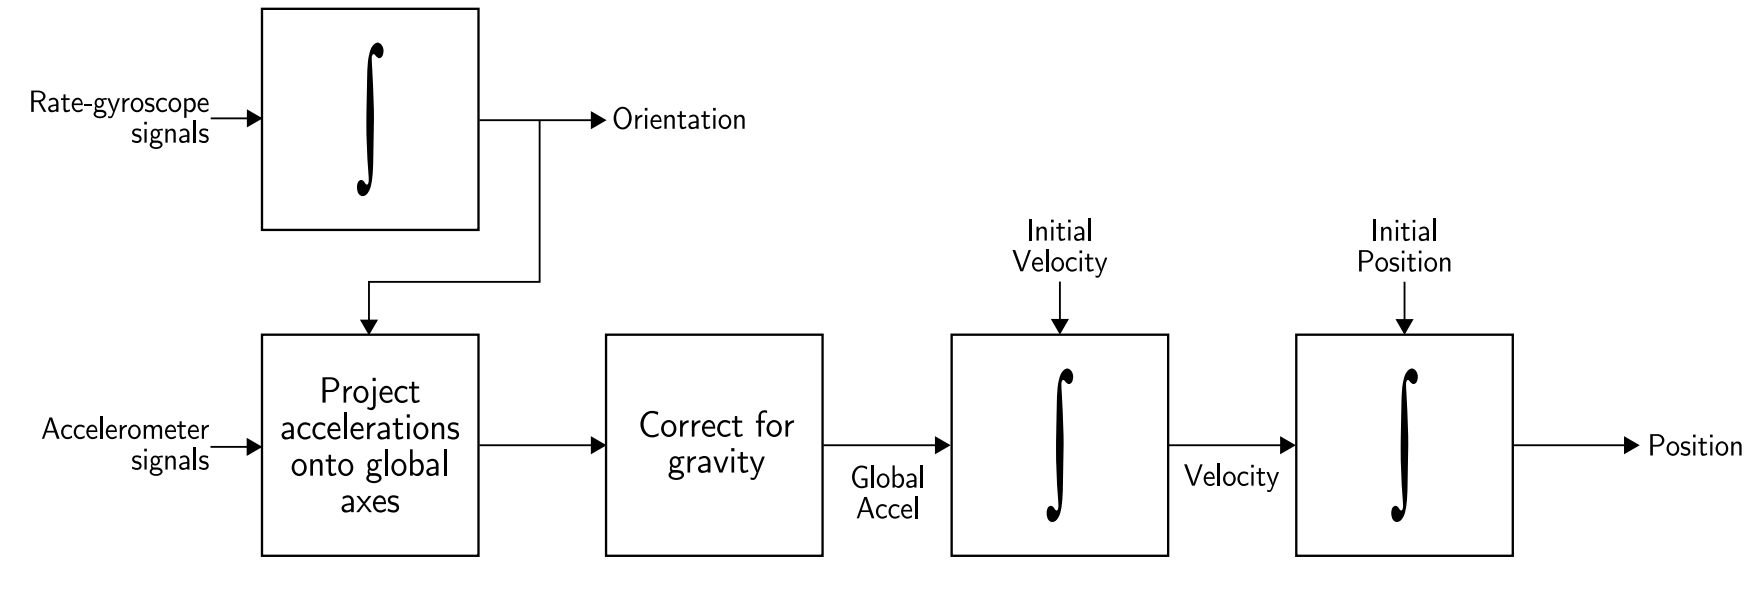
\includegraphics[scale=0.22]{images/fig_chapter1/strap_imu_algo.png}
\caption{Strap-down inertial navigation algorithm}
\label{fig:strapdown_imu}
\end{figure}

Based on the algorithm we can see that to estimate the pose, we need to do integration on Gyroscope values to get orientation. And double integration on Accelerometer values to get the position. That seems simple but the IMU readings are not ideal, they contain noises and biases \citep{woodman2007introduction} which need to be accounted for.

\subsection{Noise Models}
Sensors readings are inherent to noise. There is all kinds of noise which we have to deal with.

\subsubsection{Gyro Error Characteristics}
In table \ref{tab:gyro_error} you can see all errors in MEMS gyroscope.
% gyro error table
\begin{table}[ht]
    \centering
\begin{tabular}{ |l| L| L| } \hline
     \thead{Error Type} & \thead{Description} & \thead{Result of Integration} \\ \hline
     Bias & 
     A constant Bias epsilon & 
     Steadily growing angular error.  \[\theta(t) = \epsilon.(t)\] \\
     \hline
     White Noise & 
     White noise with some standard deviation sigma & 
     An angular random walk, whose standard deviation grows with the square root of time. 
     \[\sigma_\theta(t) = \sigma.\sqrt{\delta.t}\] \\
     \hline
     Temperature Effects & 
     Temperature dependent residual bias & 
     Any residual bias is integrated into orientation, causing an orientation error which grows linearly with time. \\
     \hline
     Calibration & 
     Deterministic errors in scale factors, alignments and gyro linearities & 
     Orientation drift proportional to the rate and duration of motion. \\
     \hline
     Bias Instability & 
     Bias fluctuations, usually modelled as a bias random walk & 
     A second order random walk. \\
     \hline
\end{tabular}
    \caption{Summary of Gyro Error Sources \citep{woodman2007introduction}}
    \label{tab:gyro_error}
\end{table}

\subsubsection{Accelerometer Error Characteristics}
In table \ref{tab:accel_error} you can see all errors in an MEMS accelerometer.
% accelerometer error table
\begin{table}[ht]
    \centering
\begin{tabular}{ |l| L| L| } \hline
     \thead{Error Type} & \thead{Description} & \thead{Result of Double Integration} \\ \hline
     Bias & 
     A constant Bias epsilon in the accelerometer's output signal. & 
     A quadratically growing position error. \[s(t) = \epsilon . \frac{t^{2}}{2}\]   \\
     \hline
     White Noise & 
     White noise with some standard deviation sigma & 
     A second order random walk. The standard deviation of the position error grows as
     \[\sigma_s(t) = \sigma . t^{\frac{3}{2}} . \sqrt{\frac{\sigma . t}{3}}\]   \\
     \hline
     Temperature Effects & 
     Temperature dependent residual bias & 
     Any residual bias causes an error in position which grows quadratically with time. \\
     \hline
     Calibration & 
     Deterministic errors in scale factors, alignments and accelerometer linearities & 
     Position drift proportional to the squared rate and duration of acceleration. \\
     \hline
     Bias Instability & 
     Bias fluctuations, usually modelled as a bias random walk & 
     A third-order random walk in position. \\
     \hline
\end{tabular}
    \caption{Summary of Accelerometer Error Sources \citep{woodman2007introduction}}
    \label{tab:accel_error}
\end{table}

\subsection{Challenges in Working with IMU}
As you can see it is not straightforward to work with IMUs, especially for absolute position estimation as the errors introduced are squared with time. This presents a lot of challenges especially for our case, as we require a precision in the range 1/10 of a mm. So, the sensor readings cannot be used directly in the inertial navigation algorithm. Generally some advanced signal processing techniques and algorithms (Kalman Filter, Extended Kalman Filter, 6 DoF Kalman Filter) are used to estimate the pose using IMU. These techniques may be good enough for some other applications, but in our case their use is not enough. The precision requirements are very high. Even if we use these algorithms, there is still a drift present which is unacceptable for this use case.

% Start: Neural Networks
\section{Neural Network Architectures Explained}
We will be using a lot of Neural Networks. The basic functioning of them is explained here.

\subsection{Multi Layer Perceptron}
Most basic ANN.

\subsection{Convolutional Neural Networks}
More advanced neural networks.

\subsection{Recurrent Neural Networks}
Neural networks with memory.

\subsection{Attention Mechanism}
Talk about attention in Neural Networks.

\subsection{Transformer Networks}
How self attention is used in Neural Networks.


\begin{equation}   
        \theta(t) = \epsilon.(t)
    \end{equation}  \\